% SVN info for this file
\svnidlong
{$HeadURL$}
{$LastChangedDate$}
{$LastChangedRevision$}
{$LastChangedBy$}

\chapter{Connessione e compattezza}
\labelChapter{Connessocompatto}

\begin{introduction}
‘‘\emph{Lisa}: Allora, dov'è mio padre?\\
\emph{Professor Frink}: Beh, sarebbe ovvio anche per l'individuo più scriteriato, laureato e con specializzazione in Topologia iperbolica, che Homer Simpson è piombato... nella terza dimensione. [...] \emph{\textbf{[disegna sulla lavagna]}} Ecco un comunissimo quadrato—\\
\emph{Commissario Winchester}: Ehi ehi, rallenta, capuepopolo!\\
\emph{Professor Frink}: —ma supponiamo di estendere il quadrato oltre le due dimensioni del nostro universo, lungo l'ipotetica asse z, qui. \emph{\textbf{[tutti sussultano]}} Così si ottiene un oggetto tridimensionale noto come “cubo”, o meglio “Frinkaedro”, in onore dello scopritore!
\begin{flushright}
	\textsc{I Simpson,} La paura fa novanta VI.
\end{flushright}
\end{introduction}
\lettrine[findent=1pt, nindent=0pt]{L}{e} due proprietà che danno il nome a questo capitolo sono estremamente importanti, in quanto sono due dei principali \textit{invarianti} studiati in topologia. Entrambe rappresentano una \textit{generalizzazione} di alcuni aspetti affrontati più o meno esplicitamente durante lo studio dell'Analisi:
\begin{itemize}
	\item Ci sono sottoinsiemi del piano i cui punti possono essere \textit{connessi} da una linea arzigogolata, una spezzata o un segmento, mente
	\item Ci sono sottoinsiemi \textit{limitati} le cui successioni di punti \textit{convergono} nel sottoinsieme.
\end{itemize}
Vedremo che la \textbf{connessione} e la \textbf{compattezza} sono definite in modo abbastanza basilare, seppur non necessariamente siano intuitive a primo acchito. Tuttavia, proprio in virtù di questa semplicità, sono applicabili in tanti contesti diversi; in particolare, la compattezza come la definiremo ci permetterà di prendere informazioni note \textit{localmente} ed estenderle in modo che valgano globalmente in tutto lo spazio.
\section{Connessione}
\begin{define}[Spazio connesso e spazio sconnesso.]~{}\\
Uno spazio topologico $X$ si dice \textbf{connesso}\index{spazio!connesso} se gli unici sottoinsiemi aperti e chiusi sono $\emptyset,\ X$.\\
Uno spazio non \textit{connesso} si dice \textbf{sconnesso} oppure \textbf{non connesso}.
\end{define}
\begin{lemming}[Condizioni equivalenti della sconnessione; Manetti, 4.2.]~{}\label{sconnesso}\\
Sono condizioni equivalenti:
\begin{enumerate}
	\item $X$ è \textit{sconnesso}.
	\item $X=A\cup B$ con $A,\ B$ aperti, non vuoti, disgiunti.
	\item $X=A\cup B$ con $A,\ B$ chiusi, non vuoti, disgiunti.
\end{enumerate}
\vspace{-3mm}
\end{lemming}
\begin{demonstration}~{}\\
$2\iff3)$ Sono equivalenti: se $A$ è aperto e disgiunto da $B$ tale che $X=A\cup B$ significa che $B=\mathcal{C}A=X\setminus A$ e dunque chiuso; analogamente per $B$ aperto si ha che $A$ è chiuso: allora $A,\ B$ chiusi e aperti propri.\\
$1\implies2)$ Esiste $\emptyset\subsetneqq A \subsetneqq X$ con $A$ aperto e chiuso. Allora basta porre $B=\mathcal{C}A=X\setminus A$: essendo il complementare di $A$ è aperto e chiuso, sono disgiunti e tali per cui $B\neq X,\ B\neq \emptyset$. $A$ e $B$ soddisfano la tesi.\\
$2\implies1)$ $A$ aperto, $B$ aperto $\implies A$ chiuso perché $A=\mathcal{C}X=X\setminus B$. Inoltre $A$ non vuoto, $B$ non vuoto $\implies A\neq X$. Dunque $A$ è aperto, chiuso e $A\neq \emptyset,\ X$ e pertanto soddisfa la tesi: esiste un sottoinsieme aperto e chiuso che non il vuoto o l'insieme stesso.
\end{demonstration}
\begin{tips}
	Il lemma \ref{sconnesso} (Manetti, 4.2) ci dice che è sufficiente trovare solo due aperti (o chiusi) che soddisfano la condizione di cui sopra per affermare la sconnessione. Viceversa, per dimostrare la connessione, dobbiamo dimostrare che per ogni coppia di aperti (o chiusi) non vuoti, la cui unione è $X$, essi non siano disgiunti.
\end{tips}
\begin{examples} Esempi di spazi topologici \textit{sconnessi} in topologia Euclidea:
	\begin{itemize}
		\item $X=\realset\setminus\left\{0\right\}=\left(-\infty,\ 0\right)\cup \left(0,\ +\infty\right)$.
		\item $X=\left[0,\ 1\right]\cup \left(2,\ 3\right)$.
	\end{itemize}
\vspace{-3mm}
\end{examples}
\begin{lemming}[Connesso è disgiunto o sottoinsieme di un aperto/chiuso; Manetti, 4.4.]~{}\label{connessodisgiuntoosottoinsieme}\\
Sia $X$ spazio topologico e $A\subseteq X$ con $A$ aperto e chiuso. Sia $Y\subseteq X,\ Y$ \textit{connesso}. Allora $Y\cap A=\emptyset$ (cioè $Y\subseteq Y\setminus A$) oppure $Y\subseteq A$.
\end{lemming}
\begin{demonstration}
Consideriamo $Y\cap A$: esso è intersezione di due aperti e chiusi per ipotesi ($Y$ è aperto e chiuso perché \textit{connesso}), cioè è aperto e chiuso. Essendo $Y$ \textit{connesso}, un suo sottoinsieme aperto e chiuso o è l'insieme vuoto oppure è l'insieme stesso, cioè $Y\cap A=\emptyset$ (cioè $Y\subseteq Y\setminus A$) oppure $Y\cap A=Y$ (cioè $Y\subseteq A)$.
\end{demonstration}
\begin{theorema}[Connessione di ${\left[0,\ 1\right]}$; Manetti, 4.6.]~{}\\
Con la topologia Euclidea, $X=\left[0,\ 1\right]$ è \textit{connesso}.
\end{theorema}
\begin{demonstration}
Supponiamo che $X=\left[0,\ 1\right]=C\cup D$ con $C,\ D$ entrambi chiusi.\\
Dobbiamo dimostrare che $C,\ D$ \textit{non} sono disgiunti, ovvero $C\cap D\neq 0$. Supponiamo sia $0\in C$ e poniamo $d=\inf D$. Essendo $D$ un chiuso, $d\in \overline{D}=D$.
\begin{itemize}
	\item Se $d=0$, $d\in C\cap D\neq \emptyset$.
	\item Se $d>0$ allora $\left[0,\ d\right)\subseteq C$ perché \textit{non sta} in $D$. Il passaggio alla chiusura mantiene l'inclusione, dunque $\left[0,\ d\right]\subseteq \overline{C}=C$. Segue che $d\in C$ e dunque $C\cap D\neq \emptyset$.
\end{itemize}
\vspace{-3mm}
\end{demonstration}
\begin{theorema}[Immagine continua di un connesso è un connesso; Manetti, 4.7.]~{}\\
	L'immagine continua di un \textit{connesso} è un \textit{connesso}:
	\begin{equation}
		\funz{f}{X}{Y}\text{ continua},\ X\text{ connesso}\implies f\left(X\right)\text{ connesso}
	\end{equation}
\vspace{-6mm}
\end{theorema}
\begin{demonstration}
	Sia $Z\subseteq f\left(X\right)$, $Z$ aperto, chiuso in $f\left(X\right)$ non vuoto. Per dimostrare che $f\left(X\right)$ sia connesso ci è sufficiente dimostrare che $Z=f\left(X\right)$: in questo modo gli unici aperti e chiusi sono i sottoinsiemi impropri:
	\begin{itemize}
		\item $Z$ aperto: $\exists A$ aperto in $Y\ \colon Z=A\cap f\left(X\right)$.
		\item $Z$ chiuso: $\exists C$ chiuso in $Y\ \colon Z=C\cap f\left(X\right)$.
	\end{itemize}
Allora:
	\begin{itemize}
	\item $f^{-1}\left(Z\right)=f^{-1}\left(A\right)\cap f^{-1}\left(f\left(X\right)\right)=f^{-1}\left(A\right)\implies f^{-1}\left(Z\right)$ è uguale alla controimmagine continua di un aperto in $Y$, cioè è uguale ad un aperto di $X$.
	\item $f^{-1}\left(Z\right)=f^{-1}\left(C\right)\cap f^{-1}\left(f\left(X\right)\right)=f^{-1}\left(C\right)\implies f^{-1}\left(Z\right)$ è uguale alla controimmagine continua di un chiuso in $Y$, cioè è uguale ad un chiuso di $X$
	\end{itemize}
Segue che $f^{-1}\left(Z\right)$ è aperto e chiuso in $X$. Notiamo inoltre che, essendo $Z\neq \emptyset$, allora $f^{-1}\left(Z\right)\neq \emptyset$: essendo $X$ \textit{connesso} per ipotesi, necessariamente $f^{-1}\left(Z\right)=X$.
\end{demonstration}
\begin{observe}
Dal teorema precedente segue che essere \textit{connesso} è una proprietà topologica! Infatti, se vale per una qualunque funzione continua $\funz{f}{X}{Y}$, allora varrà anche per omeomorfismi tra $X$ e $Y$; in particolare, si avrà per suriettività che $f\left(X\right)=Y$ connesso.
\end{observe}
\subsection{Connessione per archi}
\begin{define}[Arco.]~{}\\
Un \textbf{arco}\seeonlyindex{arco}{cammino} o \textbf{cammino}\index{cammino} $\alpha$ da un punto $x$ a un punto $y$ in uno spazio topologico $X$ è una funzione continua che parametrizza un \textit{percorso} finito fra gli estremi $x$ e $y$:
\begin{equation}
\funz{\alpha}{\left[0,\ 1\right]}{X} \text{ continua}\ \colon \alpha\left(0\right)=x,\ \alpha\left(1\right)=y
\end{equation}
\vspace{-6mm}
\end{define}
\begin{define}[Connessione per archi.]~{}\\
Uno spazio topologico $X$ si dice \textbf{connesso per archi} o \textbf{c.p.a.}\index{spazio!connesso per archi}\seeonlyindex{spazio!c.p.a.}{spazio!connesso per archi} o \textit{path-connected} se per ogni coppia di punti in $X$ esiste un arco che li collega:
\begin{equation}
\forall x,\ y\in X\ \exists \funz{\alpha}{\left[0,\ 1\right]}{X} \text{ continua}\ \colon \alpha\left(0\right)=x,\ \alpha\left(1\right)=y
\end{equation}
\vspace{-6mm}
\end{define}
\begin{theorema}[$X$ c.p.a. implica $X$ connesso; Manetti, 4.7.]
\end{theorema}
\begin{demonstration}
	Sia $X=A\cup B$, con $A,\ B$ aperti non vuoti. Vogliamo dimostrare che $A\cap B\neq \emptyset$. Essendo non vuoti, prendiamo $a\in A,\ b\in B$. In quanto $X$ è \textbf{c.p.a.}, esiste il cammino (continuo) $\funz{\alpha}{\left[0,\ 1\right]}{X}$ tale che $\alpha\left(a\right)=a,\ \alpha\left(1\right)=b$.\\
	Studiamo la controimmagine di $\alpha$:
	\begin{gather*}
		\alpha^{-1}\left(X\right)=\alpha^{-1}\left(A\cup B\right)=\left[0,\ 1\right]\\
		\left[0,\ 1\right]=\alpha^{-1}\left(A\cup B\right)=\alpha^{-1}\left(A\right)\cup \alpha^{-1}\left(B\right)
	\end{gather*}
$\alpha^{-1}\left(A\right),\ \alpha^{-1}\left(B\right)$ sono entrambi aperti e non vuoti in quanto controimmagini (continue) di aperti non vuoti ($0\in \alpha^{-1}\left(A\right),\ 1\in \alpha^{-1}\left(B\right)$).\\
Poiché $\left[0,\ 1\right]$ è connesso, allora le controimmagini trovate \textit{non} sono disgiunte. Segue allora che $\exists t\in \alpha^{-1}\left(A\right)\cap \alpha^{-1}\left(B\right)$ e quindi:
\begin{equation*}
\alpha\left(t\right)\in\alpha\left(\alpha^{-1}\left(A\right)\cap \alpha^{-1}\left(B\right)\right)\subseteq\alpha\left(\alpha^{-1}\left(A\right)\right)\cap\alpha\left(\alpha^{-1}\left(B\right)\right)=A\cap B
\end{equation*}
\vspace{-3mm}
\end{demonstration}
\begin{define}[Giunzione di cammini.]~{}\\
	Dati due cammini in uno spazio $X$:
	\begin{gather*}
		\funz{\alpha}{\left[0,\ 1\right]}{X}\quad \alpha\left(0\right)=x,\ \alpha\left(1\right)=y\\
		\funz{\beta}{\left[0,\ 1\right]}{X}\quad \beta\left(0\right)=y,\ \beta\left(1\right)=z
	\end{gather*}
	Allora possiamo creare un cammino $\alpha \ast \beta$ con la \textbf{giunzione di cammini}\index{cammino!giunzione di cammini}:
	\begin{equation}
		\left(\alpha\ast\beta\right)\left(t\right)=\begin{cases}
			\alpha\left(2t\right)\quad\text{se }0\leq t\leq \frac{1}{2}\\
			\beta\left(2t-1\right)\quad\text{se }\frac{1}{2}\leq t\leq 1\\	
		\end{cases}
	\end{equation}
\vspace{-6mm}
\end{define}
\begin{lemming}[Unione di c.p.a. non disgiunta è c.p.a.]~{}\label{unionecpa}\\
	Sia $A,\ B$ \textbf{c.p.a}, $A\cap B\neq \emptyset\implies A\cup B$ \textbf{c.p.a.}
\end{lemming}
\begin{demonstration}
	Se $x, y\in A$ oppure $x,\ y\in B$ esiste per ipotesi un arco che li collega. Dobbiamo allora trovare un arco in $A\cup B$ da $x$ a $y$ $\forall x\in A, y\in B$. Preso $z\in A\cap B$, per ipotesi esistono due cammini ad esso:
	\begin{gather*}
		\funz{\alpha}{\left[0,\ 1\right]}{A}\quad \alpha\left(0\right)=x,\ \alpha\left(1\right)=z\\
		\funz{\beta}{\left[0,\ 1\right]}{B}\quad \beta\left(0\right)=z,\ \beta\left(1\right)=z	
	\end{gather*}
	Usando la \textit{giunzione di cammini}, si ha:
	\begin{equation}
		\left(\alpha\ast\beta\right)\left(t\right)=\begin{cases}
			\alpha\left(2t\right)\quad\text{se }0\leq t\leq \frac{1}{2}\\
			\beta\left(2t-1\right)\quad\text{se }\frac{1}{2}\leq t\leq 1\\	
		\end{cases}
	\end{equation}
	Il cammino $\funz{\alpha\ast\beta}{\left[0,\ 1\right]}{A\cup B}$ è quello richiesto.
\end{demonstration}
\begin{observes}~{}\label{giunzionecpa}
	\begin{itemize}
		\item Usando la giunzione di cammini, si ha che:
		\begin{equation*}
			X\text{ è \textbf{c.p.a.}}\iff \exists z\in X\ \colon \forall x\in X\quad
			\exists \funz{\alpha}{\left[0,\ 1\right]}{X}\ \colon \alpha\left(0\right)=z,\ \alpha\left(1\right)=x
		\end{equation*}
		In altre parole, uno spazio è \textbf{c.p.a.} se e solo se esiste un punto per cui ogni altro punto è collegato tramite un arco.
		\item Per ogni arco $\alpha$ esiste l'arco inverso, percorso al contrario: $\overline{\alpha}\left(t\right)=\alpha\left(1-t\right)$.
	\end{itemize}
\vspace{-3mm}
\end{observes}
\begin{define}[Segmento.]~{}\label{segmento}\\
In $\realset^n$, un \textbf{segmento}\index{segmento} $\overline{PQ}$ è la combinazione lineare tra i punti $P$ e $Q$, parametrizzato come:
	\begin{equation}
		\overline{PQ}=\left\{P+tQ\mid t\in\left[0,\ 1\right]\right\}
	\end{equation}
\vspace{-6mm}
\end{define}
\begin{define}[Sottoinsieme convesso.]~{}\\
	Un sottoinsieme $Y\subseteq\realset^n$ è \textbf{convesso}\index{sottoinsieme!convesso} se per ogni coppia di punti esiste un segmento che li collega contenuto interamente in $Y$.
	\begin{equation}
		\forall P,\ Q\in Y\quad \overline{PQ}\subseteq Y
	\end{equation}
\vspace{-6mm}
\end{define}
\begin{define}[Sottoinsieme stellato.]~{}\\
	Un sottoinsieme $Y\subseteq\realset^n$ è \textbf{stellato}\index{sottoinsieme!stellato} per $P$ se esiste un $P\in Y$ tale che per ogni altro punto esiste un segmento che li collega contenuto interamente in $Y$.
	\begin{equation}
		\exists P \in Y\ \colon \forall Q\in Y\quad \overline{PQ}\subseteq Y
	\end{equation}
\vspace{-6mm}
\end{define}
\begin{examples}~{}
\begin{itemize}
	\item Gli intervalli aperti e semiaperti sono \textbf{c.p.a}, dunque sono \textit{connessi}: l'arco $\alpha$ è banalmente il segmento pari all'intervallo aperto.
	\item Preso $X\subseteq\realset^n$ \textit{convesso}, qualunque segmento è anche per costruzione un arco: $X$ è anche \textbf{c.p.a} e dunque \textit{connesso}.
	\item $X=\realset^{2}\setminus\left\{0\right\}$ \textit{non} è \textit{convesso} (per $\left(0,\ 1\right)$ e $\left(0,\ -1\right)$ non si hanno segmenti interni ad $X$) ma è \textbf{c.p.a.} (basta prendere un cammino che ‘‘giri attorno'' all'origine) e dunque è \textit{connesso}.
	\item Preso $X\subseteq\realset^n$ \textit{stellato} per $P\in X$, qualunque segmento con $P$ è anche per costruzione un arco: $X$ è anche \textbf{c.p.a} per l'osservazione \ref{giunzionecpa} e dunque {connesso}.
	\item Ogni insieme \textit{convesso} è anche \textit{stellato} per $P$, basta fissare un qualunque punto come nostro $P$. In generale, un insieme è convesso se e solo se è stellato per ogni suo punto.
\end{itemize}
\vspace{-3mm}
\end{examples}
\subsection{Connessione nella topologia euclidea}
Vediamo ora che conseguenze hanno questi teoremi in $\realset$ con la topologia Euclidea.
\begin{theorema}[Condizioni equivalenti della connessione su $\realset$.]~{}\\
	Sia $I\subseteq \realset$. Le seguenti affermazioni sono equivalenti:
		\begin{enumerate}
	\item $I$ è un intervallo, ovvero $I$ è \textit{convesso}.
	\item $I$ è \textbf{c.p.a.}
	\item $I$ è connesso.
		\end{enumerate}
	\vspace{-3mm}
\end{theorema}
\begin{demonstration}~{}\\
	$1) \implies 2)$ Siccome $I$ è convesso $\implies$ $I$ stellato $\implies$ $I$ \textbf{c.p.a.} $\implies$ $I$ connesso. \\
	$2) \implies 3)$ Vale in generale che \textbf{c.p.a.} $\implies$ connesso.\\
	$3) \implies 1)$ Per contronominale mostriamo che $I$ non intervallo $\implies$ $I$ sconnesso. $I$ non intervallo significa che
		\begin{gather*}
			\exists a<b<c,\ a,c\in I,\ b\notin I \\
			b\notin I \implies I= \left(\underbrace{ I\cap \left(-\infty ,b\right)}_{\in a}\ \right) \cup \left( \underbrace{I\cap \left(b ,+\infty\right)}_{\in c}\ \right)
		\end{gather*}
	ovvero $I$ è unione di aperti, non vuoti e disgiunti $\implies$ $I$ sconnesso.	
\end{demonstration}
\begin{observe}~{}\label{teorema esistenza zeri funzioni continue, s^n cpa}
		\begin{itemize}
	\item Come conseguenza immediata di questo teorema si ha il \textbf{teorema di esistenza degli zeri}\index{teorema! di esistenza degli zeri} per funzioni continue da $\realset$ in $\realset$; per tali funzioni vale che l'immagine continua di un intervallo $\left[a,\ b\right]$ è un intervallo $\left[f\left(a\right),\ f\left(b\right)\right]$, pertanto se gli estremi dell'intervallo sono tali per cui $f\left(a\right)<0<f\left(b\right)$ allora la funzione ammette uno zero, in quanto $0\in\left[f\left(a\right),\ f\left(b\right)\right]$.
	\item Per $n\geq 1$ la \textbf{sfera}\index{sfera} $\displaystyle S^n \coloneqq \left\{ \left(x_1,\ldots,x_{n+1}\right) \mid \sum_{i=1}^{n+1}x_i^2=1 \right\}$ è \textbf{c.p.a.}; infatti, $\forall x,y\in S^n$ si trova sempre un arco dato dall'intersezione di $S^n$ e del piano $H$ passante per il centro della sfera, $x$ e $y$.
		\end{itemize}
	\vspace{-3mm}
\end{observe}
Mostriamo un risultato per funzioni continue da $S^n$ in $\realset$.
\begin{theorema}[Funzioni continue da continue da $S^n$ in $\realset$.]~{}\label{non iniettività S^n in realset}\\
Sia $\funz f {S^n} \realset$ una funzione continua. Allora $\exists x\in S^n \ \colon f(x)=f(-x)$. In particolare $f$ non è iniettiva.
\end{theorema}
\begin{demonstration}
	Costruiamo una funzione $g(x)=f(x)-f(-x)$: essa è continua perché somma di funzioni continue. Siccome $S^n$ è connesso allora $g\left( S^n\right)\subseteq\realset$ è connesso $\implies$ per il teorema precedente $g\left(S^n\right)$ è un intervallo.\\
	Si considerino un punto $y\in S^n$ arbitrario e le sue immagini $g(y)$ e $g(-y)$: esse appartengono all'intervallo dell'immagine $g\left( S^n\right)$, quindi se ne può considerare il loro punto medio:
		\begin{gather*}
			\frac{1}{2}\left[ g(y) + g(-y)\right]=\frac{1}{2} \left[ f(y) -f(-y) + f(-y) -f(y) \right]= 0\\
			\implies 0\in g\left(S^n\right)\exists x\in S^n \colon g(x)=0, \text{ ovvero } f(x)=f(-x)
		\end{gather*}
	\vspace{-3mm}
\end{demonstration}
Come conseguenza di questo teorema si ha che un aperto di $\realset$ non sarà mai omeomorfo ad un aperto di $\realset^n$.
\begin{theorema}[Aperti di $\realset$ non omeomorfi ad aperti di $\realset^n$.]~{}\\
Sia $I\subseteq\realset$ e $U\subseteq\realset^n$, con $n\geq 2$. Se $I,\ U$ sono aperti allora $I$ non è omeomorfo a $U$.	
\end{theorema}	
\begin{demonstration}
	Si consideri un omeomorfismo $\funz g U I$. Siccome $U\subseteq\realset^n$ aperto allora esiste una palla aperta di raggio $\epsilon$ contenuta in $U$, se ne considera il bordo $S^n\subseteq U$. Si considera dunque la restrizione $\funz {g_{|_{S^n}}} {S^n} I$, che per il teorema precedente non è iniettiva. Dunque $g$ non è un omeomorfismo.	
\end{demonstration}

\begin{observe}
	Il teorema appena visto è un caso particolare del \textbf{teorema dell'invarianza della dimensione}\index{teorema!dell'invarianza della dimensione}: ‘‘Siano $U\subseteq\realset^n, V\subseteq\realset^m$ aperti. Se $U\cong V \implies n=m$. Equivalentemente $n\neq m\implies U\ncong V$''. A pag. \pageref{invarianzadimensionen=2} si può trovare la dimostrazione di un altro caso particolare, quello per gli aperti di $\realset^2$.
\end{observe}
% LEZ 08
\subsection{Unioni e prodotti di spazi connessi}
\begin{theorema}[Unione arbitraria di sottospazi connessi è un connesso.]~{}\label{unione sottospazi connessi}\\
Siano $\left\{ X_i \right\}_{i\in I}$ una famiglia di sottoinsiemi di uno spazio topologico $X$. Se ogni $X_i$ è connesso e $\displaystyle\bigcap_{i\in I}X_i\neq\emptyset$ allora $\displaystyle\bigcup_{i\in I}X_i$ è connesso.	
\end{theorema}
\begin{demonstration}
	Sia $\displaystyle Z\subseteq Y\coloneqq \bigcup_{i\in I}X_i$ un aperto e chiuso non vuoto. Vogliamo dimostrare che $Z=Y$, cosicché $Y$ risulti connesso. Basta mostrare l'inclusione $Y\subseteq Z$.\\
	Se considera l'intersezione di $Z$ e di un connesso fra gli $\left\{X_i\right\}$, essa sarà banale per il lemma \ref{connessodisgiuntoosottoinsieme}:
	\begin{gather*}
		X_i \cap Z = \begin{cases}
			\emptyset & \\
			X_i	&		
		\end{cases}
	\end{gather*}
	Essendo $Z\neq\emptyset$ e contenuto nell'unione $\displaystyle \bigcup_{i\in I}X_i$, $\exists i_0$ tale per cui $X_{i_0}\cap Z\neq \emptyset$, da cui segue che $X_{i_0}\cap Z=X_{i_0} \implies X_{i_0}\subseteq Z $.\\
	Siccome $\displaystyle \bigcap_{i\in I}X_i\neq\emptyset$, esisterà sicuramente $x\in\bigcap_{i\in I}X_i\subseteq X_{i_0}\subseteq Z \implies x\in Z$. Poiché $x\in X_i, \forall i$ per definizione di intersezione, segue che $\forall i\in I, \ X_i\cap Z\neq\emptyset$. Quindi, per $\forall i,\ X_i\subseteq Z \implies Y\subseteq Z \implies Y=Z$, quindi $Y$ è connesso perché l'unico aperto e chiuso non vuoto è se stesso.
\end{demonstration}
\begin{theorema}[Prodotto di connessi è connesso.]~{}\label{prodotto connessi}\\
$X, Y$ sono spazi topologici connessi $\iff X\times Y$ è connesso.	
\end{theorema}
\begin{demonstration}~{}\\
	$\impliessx$ Segue dalla continuità e suriettività delle proiezioni e dal fatto che l'immagine continua di un connesso è connessa:
		\begin{gather*}
			\funz p {X\times Y} X \text{continua e suriettiva } \implies p(X)=X \text{ connesso}\\
			\funz q {X\times Y} Y \text{continua e suriettiva } \implies q(Y)=Y \text{ connesso}	
		\end{gather*}	
	$\impliesdx$ Notiamo che, essendo $X\times\{y\}\cong X$ con $X$ connesso, al variare di $y\in Y$ abbiamo delle fibre tutte connesse che spazzano lo spazio prodotto $X\times Y$
	\begin{equation*}
		X\times Y=\bigcup_{y\in Y}X\times\{y\}
	\end{equation*}
	Tuttavia, le $X\times\{y\}$ sono tutte \textit{disgiunte} le une dalle altre e non è sufficiente per affermare la connessione di $X\times Y$!\\
	L'idea è quindi quella di creare una sorta di ‘‘guida'' \textit{connessa} la cui intersezione con le fibre $X\times\{y\}$ non sia vuota; posto $X_y=X\times\{y\}$, prendiamo $x_0\in X$ e definiamo $Y_{x_0}=\{x_0\}\times Y\cong Y$ connesso. Poichè $Z_y=X_y\cup Y_{x_0}$ è connesso $\forall y$ perché unione di connessi la cui intersezione è $\{\left(x_0,\ y\right)\}$, dalle osservazioni precedenti segue che:
		\begin{equation*}
			X\times Y=\bigcup_{y\in Y}Z_y=\bigcup_{y\in Y}\left(X_y \cup Y_{x_0}\right),\ \bigcap_{y\in Y}\left(Z_y\right)=Y_{x_0}\neq\emptyset	
		\end{equation*}
	Dunque $X\times Y$ è unione di connessi la cui intersezione non è vuota, quindi per il teorema precedente è connesso.
\end{demonstration}
\begin{attention}
	L'intersezione di connessi non è necessariamente un connesso! Prendiamo su $\realset^2$ con topologia Euclidea la circonferenza unitaria $S^1=\{\left(x,\ y\right)\in \realset^2\mid x^2+y^2=1\}$ e il segmento sull'asse $x$ dato da $[-1,\ 1]\times\{0\}$: essi sono due \textbf{c.p.a.} (e quindi connessi), ma la loro intersezione è $\{\left(-1,\ 0\right),\ \left(1,\ 0\right)\}$ che è chiaramente sconnessa.\\
	Tuttavia, ciò è vero se lo spazio è $\realset$ con la topologia Euclidea: poiché i connessi sono gli intervalli, la loro intersezione rimane comunque un intervallo (o al più un punto) che è connesso.
\end{attention}
\subsection{Spazi connessi non c.p.a.}
Approfondiamo ora la differenza fra essere spazio connesso o \textbf{c.p.a.}, mostrando esempi di un tipo ma non dell'altro. Prima, però, dimostreremo un teorema sulla caratterizzazione di un \textit{insieme denso} che ci tornerà utile.
\begin{theorema}[Caratterizzazione di un insieme denso.]~{}\\
	Sia $X$ uno spazio topologico e $A\subseteq X$ un suo sottoinsieme, allora:
		\begin{gather*}
			A \text{ è denso }\iff \forall U\subseteq X \text{ aperto e }U\neq\emptyset, \ U\cap A\neq\emptyset	
		\end{gather*}
	\vspace{-6mm}
\end{theorema}
\begin{demonstration}~{}\\
	$\impliesdx$ Se $A$ è denso allora $\overline{A}=X$. Supponiamo che $\exists V$ aperto $\colon V\cap A=\emptyset$. Siccome $V$ è aperto allora $X\setminus V$ è chiuso, inoltre $V\cap A=\emptyset$, quindi $A\subseteq X\setminus V$. Essendo $A$ contenuto in un chiuso allora lo sarà anche la sua chiusura, siccome è il più piccolo chiuso che lo contiene:
		\begin{equation*}
			A\subseteq X\setminus V \implies \overline{A}=X\subseteq \overline{X\setminus V}=X\setminus V \implies V=\emptyset
		\end{equation*}
	Ne segue che l'unico aperto che non interseca $A$ è l'insieme vuoto. \\
	$\impliessx$ Consideriamo un chiuso $K\supseteq A$. Siccome è chiuso allora il suo complementare $X\setminus K$ è aperto. Per ipotesi dunque si ha che $V\cap A\neq \emptyset$ oppure $V=\emptyset$, passando al complementare si ottiene che:
	\vspace{-1mm}
		\begin{equation*}
			\begin{array}{llllllll}
				A\subseteq K &\implies& X\setminus K \subseteq X\setminus A &\implies& V\subseteq X\setminus A &\implies& V\cap A=\emptyset&\\
				& \implies& V=\emptyset& \implies& K=X& \implies & \overline{A}=X&
			\end{array}
		\vspace{-2mm}
		\end{equation*}
	L'ultima implicazione è dovuta al fatto che ogni chiuso che contiene $A$ si è dimostrato essere solo $X$ per cui esso sarà la sua chiusura.
\end{demonstration}

\begin{theorema}[Chiusura e connessione.]~{}\label{chiusuraconnessa}\\
Sia $X$ uno spazio topologico e $Y\subseteq X$ connesso, allora:
		\begin{equation}
			\forall W \colon Y\subseteq W \subseteq \overline{Y} \implies W \text{ connesso}
		\end{equation}
	In particolare la chiusura di un connesso è connessa.
\end{theorema}
\begin{demonstration}
	Consideriamo un sottoinsieme $Z\subseteq W$ aperto, chiuso e non vuoto; dimostriamo che $Z$ deve coincidere con $W$, cioè $W$ ammette come aperto e chiuso non vuoto solo se stesso.
		\begin{gather*}
			Z\subseteq W \text{ aperto } \implies \exists A\subseteq X \text{ aperto } \colon Z=W\cap A \\
			Z\subseteq W \text{ chiuso } \implies \exists C\subseteq X \text{ chiuso } \colon Z=W\cap C
		\end{gather*}
	Studiamo adesso l'intersezione di $Z$ con $Y$:
		\begin{gather*}
			Z\cap Y=A\cap W\cap Y \stackrel{!}{=} A\cap Y \text{ aperto in Y}\\
			Z\cap Y=C\cap W\cap Y \stackrel{!}{=} C\cap Y \text{ chiuso in Y}
		\end{gather*}
	Il passaggio indicato con (!) è dovuto al fatto che $Y\subseteq W$. Poichè $Z\cap Y$ è aperto e chiuso in $Y$, se $Z\cap Y$ è non vuoto seguirà che $Y\subseteq Z$ in quanto $Y$ è connesso. Per provare che tale intersezione non è vuota utilizziamo il teorema precedente:
		\begin{gather*}
			Y \text{ denso in W, infatti } \mathcal{cl}_W(Y)=\mathcal{cl}_X(Y)\cap W=\overline{Y}\cap W=W\\
			Z \text{ aperto in } W\text{ e } Y \text{ denso in } W \implies Z\cap Y \neq \emptyset
		\end{gather*}
	Come già detto, si ha che $Z\cap Y=Y \implies Y\subseteq Z$. Poichè $Y$ è denso in $W$ e $Z$ è chiuso in $W$, il quale contiene $Y$, si ha:
		\begin{equation*}
			W=\mathcal{cl}_W(Y)\subseteq \overline{Z}=Z \implies W\subseteq Z \implies W=Z \implies W \text{ connesso}
		\end{equation*}
\vspace{-3mm}
\end{demonstration}
Vediamo ora degli esempi di spazi connessi ma non \textbf{c.p.a.}
\begin{example}\textsc{Seno del topologo.}\\
\begin{minipage}{0.47\textwidth}
Sia $Y\subseteq \realset^2$ con la topologia euclidea e $Y=\left\{ \left( x,\ \sin\frac{1}{x} \right) \mid x>0 \right\}$, detto anche \textbf{seno del topologo}\index{seno del topologo}. Esso è \textbf{c.p.a.} perché per connettere due punti basta percorrere la curva stessa del grafico. Quindi $Y$ è connesso, dunque per il teorema \ref{chiusuraconnessa} (pag. \pageref{chiusuraconnessa}) $\overline{Y}$ è connesso.\\
Tuttavia $\overline{Y}$ non è \textbf{c.p.a.} in quanto $\overline{Y}=Y\cup \left\{ (0,y) \mid -1\leq y \leq 1 \right\}$ ed i punti sull'asse delle $y$ e sulla curva $Y$ non si possono connettere tramite un arco continuo.
\end{minipage}
\hspace{-7mm}
\begin{minipage}{0.52\textwidth}
	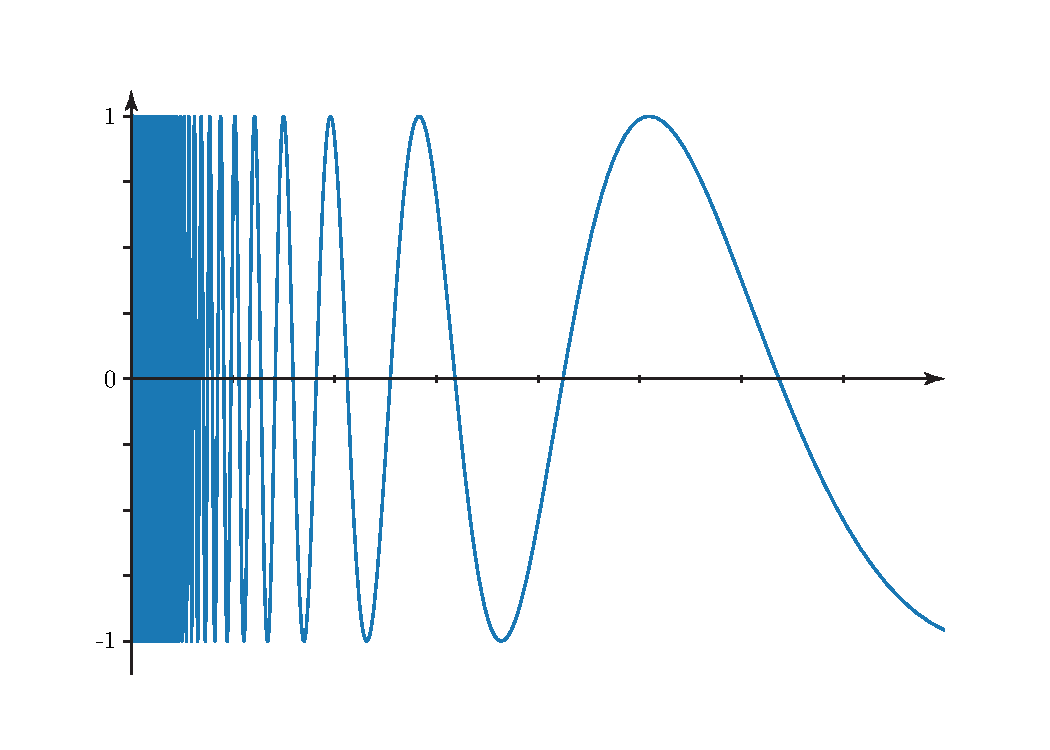
\includegraphics[trim=0cm 0.5cm 0.5cm 1.25cm,clip,scale=0.50]{images/topologistsine.pdf}
\end{minipage}
\end{example}
\begin{example}\textsc{La pulce ed il pettine.}\\
	Si consideri il ‘‘pettine'' come il seguente sottospazio di $\realset ^2$ con la topologia euclidea:
		\begin{equation*}
			Y= \left\{ (x,\ 0) \mid 0\leq x\leq 1 \right\} \cup \bigcup_{\stackrel{r\in\rationalset}{ 0\leq r\geq 1}} \left\{ (r,\ y) \mid 0\leq y \leq 1 \right\}
		\end{equation*}
\begin{minipage}{0.62\textwidth}
Presi due punti su $Y$ si possono collegare fra loro scendendo alla base del pettine $\left[0,\ 1\right]$ e risalendo sui ‘‘denti'' di ascissa razionale. Quindi $Y$ è \textbf{c.p.a.}, allora $Y$ è connesso e $\overline{Y}=\left[0,\ 1\right]\times \left[0,\ 1\right]$.\\
Si consideri ora la ‘‘pulce'', ovvero un punto $P$ di ascissa irrazionale ed ordinata 1, ad esempio $P=\left(\frac{\sqrt{2}}{2},\ 1\right)$. Sia $Z=Y\cup P$; per il teorema precedente segue che $Z$ è connesso, infatti:
\begin{gather*}
	Y\subseteq Z \subseteq \overline{Y}=\left[0,\ 1\right]\times \left[0,\ 1\right]	
\end{gather*}
	\end{minipage}
	\begin{minipage}{0.37\textwidth}
		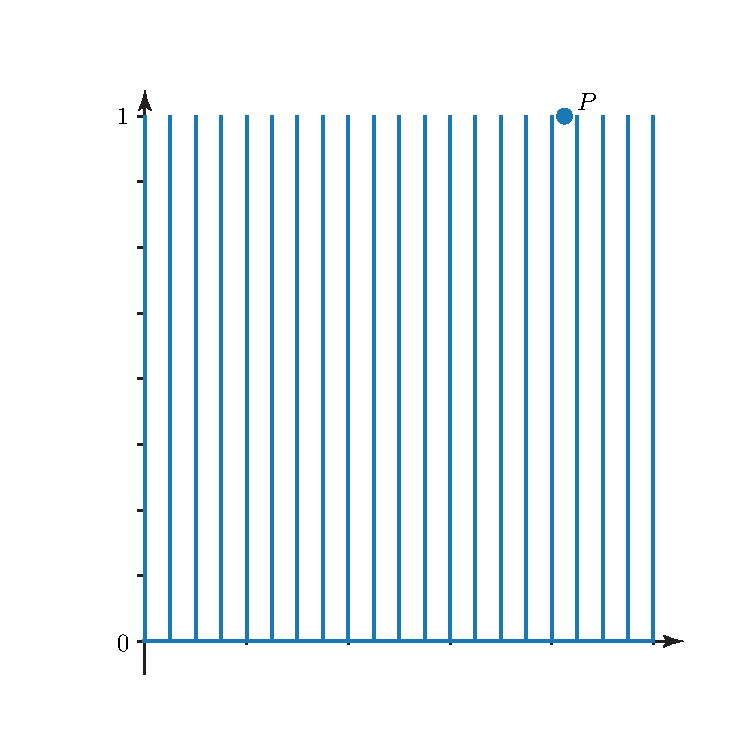
\includegraphics[trim=1.1cm 0.5cm 0.5cm 1.25cm,clip,scale=0.50]{images/comb.pdf}
	\end{minipage}\\
Tuttavia $Z$ non è \textbf{c.p.a.}: preso un cammino $\funz \alpha {\left[0,\ 1\right]} {Z\subseteq \realset^2}$ tale che $\alpha(t)= \left( x(t), y(t)\right)$ con $\alpha (0)=(0,0)$ e $\alpha(1)=P$, per continuità $y(t)\neq 0 \implies x(t)\in\rationalset$, ma \textit{non} è vero per $P$ che ha ascissa irrazionale, dunque non esiste un cammino continuo che colleghi l'origine e $P$. Ne consegue che $Z$ non è \textbf{c.p.a.}
\end{example}

\begin{theorema}[Immagine continua di uno spazio c.p.a. è un c.p.a.]~{}\\
L'immagine continua di uno spazio \textbf{c.p.a.} è \textbf{c.p.a.}:
	\begin{equation}
		\funz{f}{X}{Y}\text{ continua},\ X\textbf{ c.p.a.}\implies f\left(X\right)\textbf{ c.p.a.}
		\end{equation}
		\vspace{-6mm}
	\end{theorema}
\begin{demonstration}
	Considerati $y,\ z\in f\left(X\right)$, vogliamo trovare un cammino tra i due punti. Poiché $y,\ z\in f\left(X\right)$, consideriamo $a,\ b\in X$ tali che $y=f(a)$ e $z=f(b)$. Poichè $a,\ b\in X$ \textbf{c.p.a.}, esiste un cammino $\alpha$ tale per cui $\alpha\left(0\right)=a$ e $\alpha\left(1\right)=b$; componiamolo ora con la funzione $f$.
\[
\begin{tikzcd}
	{f\circ \alpha\ \colon \left[0,\ 1\right]} \arrow[r, "\alpha"] & X \arrow[r, "f"] & Y
\end{tikzcd}
\]
La composizione $f\circ \alpha$ è continua perché composizione di funzioni continue, inoltre:
\begin{gather*}
	\left(f\circ \alpha\right)\left(0\right)=f\left(\alpha\left(0\right)\right)=f\left(a\right)=y\\
	\left(f\circ \alpha\right)\left(1\right)=f\left(\alpha\left(1\right)\right)=f\left(b\right)=z
\end{gather*}
Dunque $f\circ \alpha$ è un cammino fra due punti $y,\ z$ arbitrari in $f\left(X\right)$ e pertanto $f\left(X\right)$ è \textbf{c.p.a.}
\end{demonstration}
\subsection{Componenti connesse}
L'intuizione geometrica che ci ha portati alla definizione di connessione è stata ‘‘di quanti pezzi è fatto uno spazio?''. Se uno spazio è connesso è fatto di un solo ‘‘pezzo'', cerchiamo ora di definire cosa sono i ‘‘pezzi'' e come sono fatti.
\begin{define}[Componente connessa.]~{}\\
	Sia $X$ uno spazio topologico e $C\subseteq X$. Si dice che $C$ è una \textbf{componente connessa}\index{componente!connessa} se:
		\begin{itemize}
			\item $C$ è \textit{connesso}.
			\item $C$ è \textbf{massimale}\index{massimale}, ovvero $C\subseteq A$, $A$ connesso $\implies C=A$.
		\end{itemize}
	Scelto $x\in X$ si può definire la \textbf{componente connessa di un punto}\index{componente!connessa di un punto}, ovvero:
	\begin{equation}
		\displaystyle C(x)=\bigcup \{C \mid C\text{ connesso},\ x\in C\}
	\end{equation}
\vspace{-6mm}
\end{define}
La componente connessa di \textit{un punto} è effettivamente una componente connessa: infatti, è connessa perché unione di connessi con intersezione \textit{non vuota} ($x$ stesso) e se $C(x)\subseteq A \implies x\in A \implies A\subseteq C(x) \implies A=C(x)$.\\
Vediamo ora qualche proprietà delle componenti connesse, in particolare che sono chiuse e formano una partizione.
\begin{theorema}[Componenti connesse sono chiuse e formano una partizione.]~{}\\
	Sia $X$ uno spazio topologico, allora:
		\begin{enumerate}
			\item le componenti connesse sono chiuse.
			\item le componenti connesse formano una partizione di $X$.
		\end{enumerate}
	\vspace{-3mm}
\end{theorema}
\begin{demonstration}
	~{}
	\begin{enumerate}[label=\Roman*]
		\item Sia $C$ una componente connessa. Per ogni insieme vale che $C\subseteq\overline{C}$, ma $C$ è connesso, quindi $\overline{C}$ è connesso. Siccome $C$ è massimale allora $C=\overline{C}$, ovvero è chiuso.
		\item Per dimostrare che le componenti connesse formano una partizione di $X$ dobbiamo mostrare che $X$ è unione disgiunta delle componenti connesse. Prima di tutto notiamo come l'unione delle componenti connesse $C\left(x\right)$ al variare dei punti $x\in X$ coprono lo spazio:
			\begin{equation*}
				\forall x\in X,\ x\in C(x) \implies X=\bigcup_{x\in X}C(x)
			\end{equation*}
		Mostriamo ora che sono disgiunte. Prendiamo due componenti connesse $C$ e $D$ e supponiamo per assurdo che non siano disgiunte; grazie alla proprietà di massimalità delle componenti connesse segue che:
		\begin{gather*}
			C\cap D\neq\emptyset \implies C\cup D \text{ connesso } \implies C=C\cup D=D
		\end{gather*}
	\end{enumerate}
\vspace{-6mm}
\end{demonstration}
\begin{example}
	Sia $\rationalset\subseteq\realset$ con la topologia Euclidea. La componenti connesse di $\rationalset$ sono i punti, quindi i punti sono chiusi in $\rationalset$, il che è una riconferma dato che sappiamo che $\rationalset$ è Hausdorff. Tuttavia non possono essere aperti altrimenti avremmo la topologia discreta!\\
	Inoltre siccome $\rationalset$ ha più di una componente connessa significa che non è connesso! Invece $\realset$ è connesso grazie all'assioma di completezza.
\end{example}
\begin{observe}
	Dati due spazi omeomorfi si ha che hanno lo stesso numero di componenti connesse in quanto l'immagine continua di connessi è connessa. Quindi il \textbf{numero di componenti connesse} ci fornisce un criterio per determinare quando due spazi non sono omeomorfi!
\end{observe}


		\section{Compattezza}
\begin{define}[Ricoprimento aperto e sottoricoprimento.]~{}\\
	Sia $X$ uno spazio topologico. Un \textbf{ricoprimento aperto}\index{ricoprimento}\index{ricoprimento!aperto} di $X$ è una famiglia $\mathcal{A}=\{A_i \}_{i\in I}$ di aperti di $X$ tali che $X=\bigcup_{i\in I} A_i$. \\
	Un \textbf{sottoricoprimento}\index{sottoricoprimento} $\mathcal{B}$ di un ricoprimento aperto $\mathcal{A}$ è una famiglia di aperti di $\mathcal{A}$ la cui unione è ancora tutto $X$.
\end{define}		

\begin{examples}\textsc{Esempi di ricoprimenti aperti.}
	\begin{itemize}
		\item $\displaystyle \realset=(-\infty ,\ 2)\cup(0,\ +\infty)$ è un ricoprimento aperto
		\item $\displaystyle \realset =\bigcup_{n\in\naturalset}(-n,\ n)$ è un ricoprimento aperto
		\item $\displaystyle \realset=\bigcup_{p \text{ primo}}(-p,p)$ è un ricoprimento aperto
	\end{itemize}
\end{examples}

\begin{define}[Spazio compatto.]~{}\\
	Uno spazio topologico $X$ si dice \textbf{compatto}\index{spazio!compatto} se dato un qualsiasi ricoprimento aperto $\mathcal{A}$ si può sempre estrarre un sottoricoprimento \textit{finito} $\mathcal{B}$.
\end{define}
L'importanza della definizione risiede nel fatto che non si chiede che esista un ricoprimento $\mathcal{A}$ finito (basterebbe banalmente $X$ stesso che è aperto) bensì che da $\mathcal{A}$ si possa sempre estrarre un \textit{numero finito di aperti} che ricopra ancora $X$.

\begin{examples}\textsc{Esempi di spazi non compatti.}
	\begin{itemize}
		\item $\realset$ con la topologia euclidea: se si considera il ricoprimento aperto $\displaystyle \realset=(-\infty , 2)\cup(0,+\infty)$, esso non ammette sottoricoprimento finito.
		\item Gli intervalli aperti o semiaperti della forma $[a,\ b)$ hanno come ricoprimento aperto $\mathcal{A}=\left\{ \left[ a, \ b-\frac{1}{n}\right) \right\}_{n\in \naturalset}$, che non ammette un sottoricoprimento finito.
	\end{itemize}
\end{examples}

\begin{theorema}[Immagine continua di un compatto è un compatto]\label{immagine compatto}
	Dati $X,Y$ spazi topologici, $\funz f X Y$ continua, allora
		\begin{gather*}
			X \text{ compatto } \implies f(X) \text{ compatto }
		\end{gather*}
	\vspace{-6mm}
\end{theorema}
\begin{demonstration}
	Sia  $\mathcal{A}=\{A_i\}$ ricoprimento aperto di $f(X)$. Per definizione di ricoprimento allora:
	\begin{equation*}
		f(X)\subseteq \bigcup_{i\in I}A_i
	\end{equation*}
	Si considerino ora le controimmagini degli aperti $A_i$ tramite $f$, aperte in quanto $f$ è continua.
	\begin{equation*}
	X\subseteq f^{-1}\left(\bigcup_{i\in I}A_i\right)=\bigcup_{i\in I}f^{-1}\left(A_i\right)
	\end{equation*}	
	Da ciò si evince che $\mathcal{A}'=\left\{f^{-1}(A_i)\right\}$ è un ricoprimento aperto di $X$; essendo $X$ compatto, si può estrarre un sottoricoprimento finito di $X$. Riapplicando la funzione $f$ troviamo un sottoricoprimento finito del ricoprimento originale:
	\begin{gather*}
		X=f^{-1}(A_1) \cup	\ldots \cup f^{-1}(A_n) \implies f(X)\subseteq A_1\cup \ldots \cup A_n \implies f(X) \text{ compatto}
	\end{gather*}
	\vspace{-6mm}
\end{demonstration}
Da questo teorema segue che essere compatti è una \textbf{proprietà topologica}.
% LEZ 09
\begin{theorema}[${[0,\ 1]}$ è un compatto.]~{}\\
	L'intervallo $[0,\ 1]\subseteq\realset$ con la topologia euclidea è compatto.
\end{theorema}
\begin{demonstration}
	Sia $\mathcal{A}=\{ A_i\}_{i\in I}$ un ricoprimento aperto di $[0,\ 1]$ con $A_i$ aperti in $\realset$.
	Sia $X=\{ t\in\realset \mid [0,t] \text{ è coperto da un numero finito di } A_i \}$. Questo insieme \textit{non} è vuoto; infatti, per $t=0$:
		\begin{gather*}
			[0,\ t]=[0,\ 0]=\{0\}\implies\exists A_0\in\mathcal{A}\colon \{0\}\subseteq A_{0} \implies 0\in X\implies X\neq\emptyset
		\end{gather*}
	Siccome $X$ non è vuoto, per la completezza dei reali ne posso considerare l'estremo superiore $b=\sup X$. Ci sono due casi, $b>1$  e $b\leq 1$: dimostriamo che il primo è possibile mentre il secondo è assurdo per definizione di estremo superiore:
		\begin{itemize}
			\item $b>1$: $\exists t\in X \colon 1<t<b \implies [0,\ 1]\subseteq [0,\ t] \subseteq A_1\cup \ldots \cup A_n$
			\item $b\leq 1$: $b\in [0,\ 1] \implies \exists A_0\in\mathcal{A} \colon b\in A_0$ con $A_0$ aperto; per definizione della topologia Euclidea esisterà una palla aperta centrata $b$ contenuta in $A_0$:
			\begin{equation*}
				\exists \delta >0 \colon B_\delta (b)=(b-\delta, \ b+\delta )\subseteq A_0
			\end{equation*}
			Sia $0<h<\delta$. Consideriamo $b+h$ e l'intervallo $[0,\ b+1]$:
				\begin{gather*}
					[0,\ b+h]=[0,\ t]\cup [t,\ b+h]\subseteq \underbrace{A_1\cup\ldots\cup A_n}_{t\in X}\cup \underbrace{A_0}_{B_\delta (b)\subseteq A_0}
				\end{gather*}	
			Quindi $b+h$ è coperto da un numero finito di aperti, pertanto $b+h\in X$, il che è assurdo perché $b=\sup X$.
		\end{itemize}
	 Segue che solo il caso $b>1$ è lecito, da cui si ha che $[0,\ 1]$ è coperto da un numero finito di aperti del ricoprimento iniziale e quindi è compatto.
\end{demonstration}
Notiamo che questo teorema implica che un intervallo $[a,\ b]\subseteq\realset$ è compatto, essendo omeomorfo a $[0,\ 1]$.\\
Vediamo ora un esempio di spazio compatto che non abbia la topologia euclidea.
\begin{example}
	Uno spazio $X$ con la \textbf{topologia cofinita} $CF$ è compatto.\\
	Ricordiamo che gli aperti nella topologia $CF$ sono i sottoinsiemi il cui complementare è finito, quindi gli aperti sono pari a $X$ privato di un numero finito di punti.\\
	Preso un ricoprimento aperto $\mathcal{A}=\{A_i\}$, scegliamo un aperto $A_0=X\setminus\{x_1,\ \ldots,\ x_n\}$. Per ricavare un sottoricoprimento finito di $\mathcal{A}$ è sufficiente considerare, per ogni punto $x_i$ che \textit{non} appartiene all'aperto $A_0$, un aperto del ricoprimento che lo contenga. In questo modo $X=A_0\cup A_1\cup A_n$ e quindi $X$ è compatto
\end{example}
\begin{observe}
Notiamo che se $X$ è \textbf{finito} allora $X$ è compatto per \textit{qualsiasi} topologia: poiché la sua cardinalità è finita, la sarà anche quella del suo \textit{insieme delle parti}, da cui scelgo gli aperti della topologia; un qualunque ricoprimento sarà necessariamente finito. I casi interessanti di spazi compatti sono quelli il cui insieme di sostegno \textit{non è finito}.\\
Inoltre, se $X$ ha la topologia \textbf{discreta} vale anche il \textit{viceversa}:
	\begin{gather*}
		X \text{ top. discreta } \implies \left( X \text{ compatto } \iff X \text{ finito}\right)
	\end{gather*}
$\impliesdx$ Consideriamo il ricoprimento aperto $\mathcal{A}=\left\{ A_x\right\}_{x\in X}$, con $A_x\coloneqq \{x\}$ aperti in quanto $X$ ha la topologia discreta. Siccome $X$ è compatto allora esiste un sottoricoprimento finito, ovvero un numero finito di aperti di $\mathcal{A}$ che ricopre $X$, ossia:
\begin{equation*}
	X=\{x_1\}\cup\{x_2\}\cup\ldots\{x_n\}\implies X={x_1,\ x_2,\ \ldots,\ x_n}\implies X \text{ finito.}
\end{equation*}
\vspace{-6mm}
\end{observe}
\subsection{Relazioni fra compattezza e altre proprietà topologiche}
\begin{theorema}[Chiuso in un compatto è compatto; Manetti, 4.41.1.]~{}\label{chiuso in compatto}\\
Un chiuso in un compatto è un compatto, ovvero se $X$ è uno spazio topologico compatto, $C\subseteq X$ chiuso allora $C$ è compatto.
\end{theorema}
\begin{demonstration}
	Sia $\mathcal{A}=\{A_i \}_{i\in I}$ un ricoprimento di $X$, sia $C\subseteq X$ chiuso, allora $A\coloneqq X\setminus C$ è aperto in $X$.\\
	Sia $\mathcal{A}'=\{A_i,\ A\}$ ricoprimento aperto di $X$. Siccome $X$ è compatto esiste un suo sottoricoprimento finito
		\begin{gather*}
			X=A_1\cup\ldots\cup A_n\cup A \implies C=X\setminus A=A_1\cup\ldots\cup A_n
		\end{gather*}
	ovvero $C$ è compatto.
\end{demonstration}

\begin{lemming}[Unione finita di compatti è un compatto; Manetti, 4.41.2.]
\end{lemming}
\begin{demonstration}
Preso un ricoprimento aperto $\mathcal{A}$ di $K_1\cup\ldots\cup K_n$, estraiamo un sottoricoprimento finito $\widetilde{\mathcal{A}}_i$ per ogni $K_i$ compatto: l'unione $\widetilde{\mathcal{A}}_1\cup\ldots\cup \widetilde{\mathcal{A}}_n$ è un sottoricoprimento finito di $\mathcal{A}$ che copre $K_1\cup\ldots\cup K_n$.
\end{demonstration}
% Vediamo ora una relazione importante fra due proprietà topologiche: compattezza e \textbf{Hausdorff}.
\begin{theorema}[Compatto in un Hausdorff è chiuso; Manetti, 4.48.]~{}\label{compatto in hausdorff chiuso}\\
Se $X$ è di Hausdorff e $K\subseteq X$ è compatto, allora $K$ è chiuso.
\end{theorema}
\begin{demonstration}
	Per dimostrare che $K$ è chiuso mostriamo che il suo complementare è aperto, in particolare mostrando che sia intorno di ogni suo punto.
	Allora, fissato un $x_0$ arbitrario nel complementare, dovrà esistere un aperto contenente $x_0$ (che può coincidere o meno con $X\setminus K$) disgiunto da $K$.
		\begin{equation*}
				K \text{ chiuso } \iff X\setminus K \text{ aperto } \iff \exists A\subseteq X\setminus K \text{ con } A \text{ aperto } \colon x_0\in A \iff A\cap K=\emptyset
		\end{equation*}
	Per ipotesi $X$ è di \textbf{Hausdorff}; fissato $x_0$ in $X\setminus K$, per ogni $y\in K$ chiaramente $x\neq y$, dunque esisteranno due intorni (aperti) $U_y\in I(x_0)$ e $V_y\in I(y)$ (dipendenti da $y$) tali che $U_y\cap V_y=\emptyset$. Consideriamo allora, al variare di $y$, l'unione di tutti gli intorni (aperti) $V_y$:
	\begin{equation*}
			V=\bigcup_{y\in K}V_y \implies K\subseteq V
	\end{equation*}
	Gli aperti $\{V_y\}$ formano un ricoprimento di $K$, dunque, essendo $K$ compatto, estraiamo un sottoricoprimento $V_{y_1}\cup\ldots\cup V_{y_n}$.\\
	Consideriamo allora gli intorni aperti di $x_0$ definiti in precedenza e selezioniamo quelli dati da $y_1,\ \ldots,\ y_n$. Sia:
	\begin{equation*}
		U=U_{y_1}\cap\ldots\cap U_{y_n} \in I(x_0)
	\end{equation*}
	Gli aperti $V$ e $U$ per costruzione \textit{non} si intersecano ($V\cap U=\emptyset$), in particolare $V\cap K=\emptyset$ perché $K\subseteq V$. Allora, per le osservazioni iniziali $U\subseteq X\setminus K$, cioè $X\setminus K$ è intorno di $x_0$. Per l'arbitrarietà di $x_0$, segue che $X\setminus K$ è aperto e quindi $K$ chiuso.
\end{demonstration}

\begin{theorema}[Compatto in $\realset$ se e solo chiuso e limitato; Manetti, 4.42.]~{}\label{compatto chiuso e limitato R}\\
Un sottospazio $K\subseteq \realset$ è compatto $\iff K$ chiuso e limitato.
\end{theorema}
\begin{demonstration}~{}\\
	$\impliesdx$ Siccome $\realset$ è di \textbf{Hausdorff} e $K$ è compatto allora per il teorema precedente $K$ è chiuso.\\
	Per vedere che è limitato consideriamo un ricoprimento aperto $\mathcal{A}=\left\{ (-n,\ n)\cap K\right\}_{n\in\naturalset}$ di $K$. Siccome è compatto allora esiste un sottoricoprimento finito, ovvero:
	\begin{gather*}
		K\subseteq (-n_1,\ n_1)\cup\ldots\cup(-n_m,\ n_m) \implies K\subseteq (-M,\ M), \ M\coloneqq \max n_i
	\end{gather*}
	quindi $K$ è limitato. \\
	$\impliessx $ $K$ è limitato, quindi $K\subseteq [-n, \ n]$ che è compatto; poiché $K$ è chiuso per ipotesi e contenuto in un compatto, per il teorema \ref{chiuso in compatto} è anch'esso compatto.
\end{demonstration}
\begin{attention}
	Il teorema precedente \textit{non} afferma che gli unici compatti di $\realset$ sono gli intervalli chiusi e limitati! Anche una loro \textit{unione finita} (anche disgiunta) potrebbe esserlo.
\end{attention}

\begin{theorema}[Funzione su compatto in $\realset$ ammette massimo/minimo; Manetti, 4.43.]~{}\label{weierstrass}\\
Sia $\funz f X \realset$ con $X$ compatto e $\realset$ con la topologia euclidea. Se $f$ è continua allora ammette massimo e minimo.
\end{theorema}
\begin{demonstration}
	$f$ continua e $X$ compatto $\implies f(X)$ compatto, e per il teorema precedente ciò equivale al fatto che $f(X)$ è chiuso e limitato.
	\begin{equation*}
		\left.
		\begin{array}{lcl}
			f\left(x\right)\text{ limitata}&\implies& \sup \left\{f\left(x\right)\right\}<+\infty\\
			f\left(x\right)\text{ chiusa}&\implies& \sup \left\{f\left(x\right)\right\}=\max \left\{f\left(x\right)\right\}\\
		\end{array}
		\right\}
		\implies f\left(x\right)\text{ ammette massimo.}
	\end{equation*}
	Analoga è la dimostrazione per il minimo.
\end{demonstration}

\begin{attention}
	Per poter parlare di massimo e minimo di una funzione c'è bisogno di un \textit{ordinamento} sul codominio; il dominio $X$ potrebbe anche non averne uno!
\end{attention}
Vogliamo ora vedere come si comporta la compattezza rispetto al prodotto, prima però va dimostrato un lemma che ci tornerà utile nella dimostrazione del teorema.
\begin{lemming}[Tube lemma.]~{\label{tube lemma}}\\
Siano $X,Y$ spazi topologici con $Y$ compatto, $x_0\in X$, $A\subseteq X\times Y\colon A$ aperto e $\{x_0\}\times Y\subseteq A$. Allora $\exists U\subseteq X$ con $x_0\in U$, aperto tale che $\{x_0\}\times Y \subseteq U\times Y \subseteq A$
\end{lemming}
\begin{demonstration}
	L'aperto $A$ si può esprimere come unione di aperti della base della topologia prodotto:
	\begin{equation*}
		A\text{ aperto in }X\times Y\implies A=\bigcup_{i\in I}\left( U_i\times V_i \right)
	\end{equation*}
	Con $U_i\subseteq X$, $V_i\subseteq Y$. $\mathcal{U}=\{U_i\times V_i\}$ è un ricoprimento di $\{x_0\}\times Y$; poiché $\{x_0\}\times Y$ è compatto in quanto omeomorfo a $Y$, esiste un suo sottoricoprimento finito da $\mathcal{U}$:
	\begin{equation*}
		\{x_0\}\times Y\subseteq (U_1\times V_1)\cup\ldots\cup (U_n\times V_n)
	\end{equation*}
	%Se necessario si eliminano gli aperti che sono disgiunti da $\{x_0\}\times Y$
	Poniamo $U=U_1\cap\ldots\cap U_n$:
	\begin{equation*}
		\{x_0\}\times Y\subseteq U\times Y \subseteq (U_1\times V_1)	\cup\ldots\cup (U_n\times V_n) \subseteq A
	\end{equation*}
	$U$ è l'aperto che soddisfa la tesi.
\end{demonstration}
\begin{theorema}[Prodotto di compatti è compatto; Manetti, 4.49.2.]~{}\label{prodotto compatti}\\
$X,Y$ compatti $\iff X\times Y$ è compatto.
\end{theorema}
\begin{demonstration}~{}\\
	$\impliessx $ Le proiezioni $p$ e $q$ sono funzioni continue e suriettive. Poiché $X\times Y$ compatto e $p\left(X\times Y\right)=X$ e $q\left(X\times Y\right)=Y$, allora $X,\ Y$ sono compatti. \\
	$\impliesdx $ Sia $\mathcal{A}=\{A_i\}$ un ricoprimento aperto di $X\times Y$. Per ipotesi $Y$ è compatto, dunque per ogni $x$ si ha $\{x\}\times Y$ compatto in quanto $\{x\}\times Y\cong Y$.
	Estraiamo un sottoricoprimento finito da $\mathcal{A}$ che copra $\{x\}\times Y$:
	\begin{equation*}
		\{x\}\times Y\subseteq A_{x,1}\cup\ldots\cup A_{x,n}=A_x
	\end{equation*}
	Gli $A_{x_i}$ dipendono dal punto $x$ scelto. Poiché $A_x$ è aperto, Per il \textit{Tube lemma} allora:
		\begin{gather*}
			\exists U_x\subseteq X \text{ aperto }\colon \{ x\}\times Y \subseteq U_x\times Y \subseteq A_x=A_{x,1}\cup\ldots\cup A_{x,n}
		\end{gather*}
	Al variare di $x\in X$ si ha un ricoprimento $\mathcal{U}=\left\{U_x\right\}_{x\in X}$ di $X$ compatto, dunque possiamo estrarne un sottoricoprimento finito $X=U_{x_1}\cup\ldots\cup U_{x_m}$. Usando la proiezione sulla componente $X$:
		\begin{equation*}
			\begin{array}{ll}
				X\times Y &= p^{-1}(X)=p^{-1}\left( U_{x_1}\cup\ldots\cup U_{x_m}\right)= (U_{x_1}\times Y)\cup\ldots\cup (U_{x_m}\times Y)\\ &\subseteq A_{x_1}\cup\ldots\cup A_{x_m} 
				\subseteq \left( A_{x_1 , 1}\cup\ldots\cup A_{x_1, n_1}\right) \cup\ldots\cup \left( A_{x_m, 1}\cup\ldots\cup A_{x_m, n_m} \right)
			\end{array}
		\end{equation*}
	Poichè $X\times Y$ è coperto da un unione finita di un unione finita di aperti del ricoprimento $\mathcal{A}$, segue che è compatto.
\end{demonstration}
Noto che il prodotto di compatti è compatto, possiamo generalizzare la caratterizzazione dei compatti in $\realset$ (teorema \ref{compatto chiuso e limitato R} al caso dello spazio $\realset ^n$.
\begin{theorema}[Compatto in $\realset^n$ se e solo chiuso e limitato; Manetti, 4.42.]~{}\label{compatto chiuso e limitato R^n}\\
$K\subseteq \realset^n$ compatto $\iff K$ chiuso e limitato.
\end{theorema}
\begin{demonstration}~{}\\
	$\impliesdx$ $K$ è compatto in $\realset^n$ che è un Hausdorff, quindi $K$ è chiuso per il teorema \ref{compatto in hausdorff chiuso}. Per dimostrare che è limitato consideriamo un ricoprimento di palle aperte centrate nell'origine e utilizziamo l'ipotesi di $K$ compatto:
		\begin{gather*}
			K\subseteq \bigcup_{n\in\naturalset} B_n(\mathbf{0}) \implies K\subseteq B_{n_1}(\mathbf{0})\cup\ldots\cup B_{n_m}(\mathbf{0}) \subseteq B_M (\mathbf{0})
		\end{gather*}
	Con $M=\max n_i$.\\
	$\impliessx$ $K$ è limitato, quindi $K\subseteq [-a,\ a]^n$ che è compatto perché prodotto di compatti, ma $K$ è anche chiuso, quindi per il teorema \ref{chiuso in compatto} è compatto.
\end{demonstration}
\begin{digression}
In realtà vale un teorema più generale, che si dimostrerà poi nel corso di \textit{Istituzioni di Analisi}.\\
\textsc{Teorema:} Sia $X$ uno spazio metrico completo, allora $K\subseteq X$ compatto $\iff K$ chiuso e \textbf{totalmente limitato}\index{spazio!totalmente limitato}, cioè $\forall\epsilon >0, \ K$ è contenuto in un'unione finita di palle di raggio $\epsilon$.\\
In $\realset^n$ vale limitato $\iff$ totalmente limitato, ma in generale no; ad esempio, consideriamo lo spazio metrico delle funzioni continue su $[0,\ 1]$ con distanza dell'estremo superiore:
	\begin{gather*}
		\mathcal{C}\left( [0, \ 1] \right) \coloneqq \left\{ \funz f {[0,\ 1]} \realset \mid f \text{ continua } \right\},  \ \ \text{con } \mvf{d}{f}{g} =\sup_{x\in [0, \ 1]} |f(x)-g(x)|
	\end{gather*}
La palla di centro l'origine $0$ e raggio $1$:
\begin{equation*}
	B_1(\mathbf{0})=\left\{ \funz f {[0,\ 1]} \realset \mid f \text{ continua }, -1\geq f(x) \leq 1 \ \right\}
\end{equation*}
È chiusa e limitata, tuttavia in $\mathcal{C}\left( [0, \ 1] \right)$ non è compatta.
\end{digression}
\begin{theorema}[Funzione continua da compatto ad Hausdorff è chiusa; Manetti, 4.52.]~{}\label{da compatto in T_2 è chiuso}
Se $\funz f X Y$ continua con $X$ è compatto e $Y$ di \textbf{Hausdorff}, allora $f$ è chiusa.
\end{theorema}
\begin{demonstration}
	Per mostrare che $f$ è chiusa consideriamo $C\subseteq X$ chiuso e mostriamo che $f(C)$ è chiuso usando i teoremi \ref{chiuso in compatto}, \ref{immagine compatto} e \ref{compatto in hausdorff chiuso}:
		\begin{equation*}
				C\subseteq X \text{ chiuso in compatto} \implies C \text{ compatto} \implies f(C) \text{ compatto in }\mathbf{T2} \implies f(C) \text{ chiuso}
		\end{equation*}
\end{demonstration}
In generale vale il \textbf{teorema di Kuratowsi-Mròwka}: $Y$ è compatto se e solo se per qualsiasi spazio topologico $X$ la proiezione $\funz {p_X} {X\times Y} X$ è chiusa; noi ne dimostreremo una versione più debole.
% LEZ 10
\begin{theorema}[Prodotto con compatto implica proiezione chiusa; Manetti, 4.49.1.]~{}\\
Siano $X,\ Y$ spazi topologici con $Y$ compatto, allora la proiezione $\funz p {X\times Y} X$ è chiusa.
\end{theorema}
\begin{demonstration}
	Preso un $C\subseteq X\times Y$ chiuso vogliamo mostrare che $p(C)\subseteq X$ è chiuso. Per far ciò, mostriamo che il suo complementare $X\setminus p(C)$ è aperto in quanto intorno di ogni suo punto.\\
	Chiaramente, se $p(C)=X$ allora è già chiuso; se invece $p(C)\neq X$ allora $\exists x_0\in X\setminus p(C)$. Si consideri la fibra di $x_0$ tramite la proiezione $p$:
		\begin{gather*}
			p^{-1}(\{x_0\} )=\{x_0\}\times Y \subseteq (X\times Y)\setminus C
		\end{gather*}
	Con $(X\times Y)\setminus C$ aperto perché complementare in $X\times Y$ del chiuso $C$. Si rientra nelle ipotesi del \textit{Tube lemma}:
		\begin{equation*}
			\exists U\subseteq X \text{ aperto } \colon \{x_0\}\times Y \subseteq U\times Y\subseteq (X\times Y)\setminus C		\end{equation*}
	Poiché la proiezione è continua, si ha:
	\begin{equation*}
		\begin{array}{ll}
			p^{-1}(U)=U\times Y\subseteq (X\times Y)\setminus C &\implies p^{-1}(U)\cap C=\emptyset \\
			& \implies U\cap p(C)=\emptyset \implies x_0\in U\subseteq X\setminus p(C)
		\end{array}	
	\end{equation*}
Segue dunque che $X\setminus p\left(C\right)$ è intorno di $x_0$. Poiché questo è vero $\forall x_0\in X\setminus p\left(C\right)$, $X\setminus p\left(C\right)$ è intorno di ogni suo punto, quindi aperto. Segue pertanto la tesi.
\end{demonstration}